% Ce stage s'inscrit dans la thématique de l'ordonnancement temps réel où l'objectif est d'assurer le
% respect des contraintes fonctionnelles et temporelles d'un système de tâches (application)
% constituant un système embarqué critique.
% Le projet SHRIMP a pour objectif de développer un ordonnanceur temps réel en ligne, global,
% praticable et efficace pour des plateformes disposant de clusters de cœurs aux architectures et
% performances hétérogènes tel que le SoC RK3399 (clusters ARM Cortex-A53 et -A72). Une thèse
% est en cours sur le sujet et vise à développer un ordonnanceur de cette catégorie sur le plan
% théorique. Les résultats théoriques optimaux existants [1,2] sont évalués par simulation et
% apparaissent comme étant peu adaptés (coût des migrations et plan d'exécution statique) et
% réalistes (hypothèse de temps continu) pour une implémentation sur une plateforme réelle. Il est
% donc important de pouvoir évaluer les solutions développées dans le projet sur de vraies cartes
% de développement disposant de processeurs multi-cœur répondant aux caractéristiques citées
% plus tôt

%section : contexte d'ou se place mon stage

Les systèmes avioniques sont habituellement des ensembles complexes reposant sur des architectures anciennes de par le niveau de certification exigé. Par conséquent, les architectures plus récentes nécessitent une phase d'étude afin d'en évaluer l'intérêt. Dans ce contexte, le projet SHRIMP a pour but d'étudier l'implémentation d'un algorithme d'ordonnancement sur une plateforme hétérogène.   

\subsection{Ordonnancement}

L'ordonnancement est l'étude de l'affectation des ressources à des tâches. Dans le cadre de mon stage, les ressources sont des processeurs et les tâches sont des programmes. L'ordonnancement consiste donc à affecter des processeurs à des programmes ou des tâches.


\subsubsection{Ordonnancement temps réel}
Dans le cas de l'ordonnancement temps réel, les tâches sont des tâches temps réel, c'est à dire des tâches qui possèdent une contrainte temporelle. Cette contrainte peut être une échéance ou un délai maximal d'exécution. L'ordonnancement temps réel est donc l'étude de l'affectation des ressources tout en garantissant le respect des contraintes temporelles des tâches. 

On peut alors définir plusieurs catégories de temps réel :
\begin{itemize}
    \item Le temps réel dur : les contraintes temporelles doivent être respectées sous peine de défaillance du système
    \item Le temps réel mou ou souple : les contraintes temporelles doivent être respectées mais une violation de ces contraintes n'entraîne pas de défaillance du système
    \item Le temps réel ferme : les contraintes temporelles doivent être respectées mais une violation de ces contraintes entraîne une dégradation des performances du système
\end{itemize}


On pourra par la suite représenter l'ordonnancement temps réel par un diagramme de Gantt. Un diagramme de Gantt est un diagramme qui représente l'utilisation des ressources en fonction du temps. On peut alors représenter l'exécution des tâches au cours du temps, en représentant leur réveil par une fleche montante, leur exécution par un rectangle, leur échéance ou \textit{deadline} par une fleche vers le bas, et la fin de leur exécution par un "T". 

\begin{figure}[H]
    \centering
    \begin{tikzpicture}[xscale=0.5, yscale=0.6]

        \newcommand\duration{15}
        \newcommand\TaskNum{2}

        % Define task properties

        \newcommand{\rectangles}[5]{
            \expandafter\def\csname rect#1ROW\endcsname{#2}
            \expandafter\def\csname rect#1START\endcsname{#3}
            \expandafter\def\csname rect#1END\endcsname{#4}
            \expandafter\def\csname rect#1COLOR\endcsname{#5}
        }

        \newcommand{\wakeup}[3]{
            \expandafter\def\csname wakeup#1ROW\endcsname{#2}
            \expandafter\def\csname wakeup#1TIME\endcsname{#3}
        }

        \newcommand{\deadline}[3]{
            \expandafter\def\csname deadline#1ROW\endcsname{#2}
            \expandafter\def\csname deadline#1TIME\endcsname{#3}
        }

        \newcommand{\execEnd}[3]{
            \expandafter\def\csname execEnd#1ROW\endcsname{#2}
            \expandafter\def\csname execEnd#1TIME\endcsname{#3}
        }
        
        
        
        \rectangles{0}{0}{0}{2}{"red"}
        \rectangles{1}{0}{5}{7}{"red"}
        \rectangles{2}{0}{10}{12}{"red"}
        
        \rectangles{3}{1}{2}{5}{"red"}
        \rectangles{4}{1}{7}{8}{"red"}
        
        
        
        \wakeup{0}{0}{0}
        \wakeup{1}{1}{0}
        \wakeup{4}{0}{5}

        \wakeup{5}{0}{5}
        \wakeup{2}{0}{5}
        \wakeup{3}{0}{10}

        \deadline{0}{0}{5}
        \deadline{1}{0}{5}
        \deadline{2}{0}{5}
        \deadline{3}{0}{10}
        \deadline{4}{0}{15}
        \deadline{5}{1}{15}

        \execEnd{0}{0}{2}
        \execEnd{1}{0}{7}
        \execEnd{2}{0}{12}
        \execEnd{3}{1}{8}        
        
        
        \foreach \rect in {0,...,4}{
            \pgfmathsetmacro{\row}{\csname rect\rect ROW\endcsname}
            \pgfmathsetmacro{\start}{\csname rect\rect START\endcsname}
            \pgfmathsetmacro{\end}{\csname rect\rect END\endcsname}
            \pgfmathsetmacro{\color}{\csname rect\rect COLOR\endcsname}

            \draw[fill=\color!30] (\start,1.5*\TaskNum - 0.5 - 1.5*\row) rectangle (\end,1.5*\TaskNum -1.5 - 1.5*\row) node[midway] {};
        }

        \foreach \wake in {0,...,5}{
            \pgfmathsetmacro{\row}{\csname wakeup\wake ROW\endcsname}
            \pgfmathsetmacro{\time}{\csname wakeup\wake TIME\endcsname}
            
            \draw[stealth-, thick] (\time,1.5*\TaskNum - 0.5 - 1.5*\row + 0.15) -- (\time,1.5*\TaskNum -1.5 - 1.5*\row) node[midway, left] {};
        }

        \foreach \dead in {0,...,5}{
            \pgfmathsetmacro{\row}{\csname deadline\dead ROW\endcsname}
            \pgfmathsetmacro{\time}{\csname deadline\dead TIME\endcsname}
            
            \draw[-stealth, thick] (\time,1.5*\TaskNum - 0.5 - 1.5*\row) -- (\time,1.5*\TaskNum -1.5 - 1.5*\row-0.15) node[midway, left] {};
        }

        \foreach \end in {0,...,3}{
            \pgfmathsetmacro{\row}{\csname execEnd\end ROW\endcsname}
            \pgfmathsetmacro{\time}{\csname execEnd\end TIME\endcsname}
            
            \draw[|-, thick] (\time,1.5*\TaskNum - 0.5 - 1.5*\row + 0.15) -- (\time,1.5*\TaskNum -1.5 - 1.5*\row) node[midway, left] {};
        }
        
        
        % Axes
        \draw[->] (0,0) -- (\duration + 1,0) node[right] {Temps};
        \draw[->] (0,0) -- (0,\TaskNum*1.5) node[above] {Taches};
        
        % Time ticks
        \foreach \x in {0,1,...,\duration}
            \draw (\x,0.1) -- (\x,-0.1) node[below] {\x};
        
            \node[left] at (-0.5,2) {$\tau_1(WCET=2,T=5)$};
            \node[left] at (-0.5,0.5) {$\tau_2(WCET=4,T=15)$};

    \end{tikzpicture}   
    
    \vspace{20pt}

    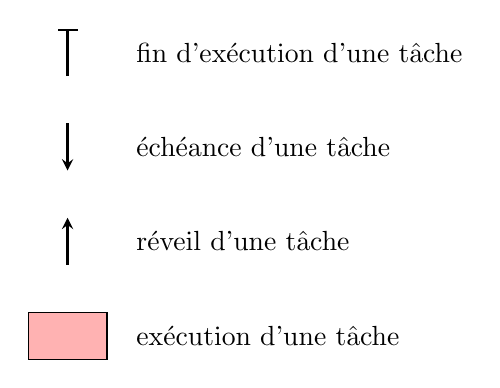
\begin{tikzpicture}[xscale=0.5, yscale=0.6, centered]
        \draw[fill=red!30] (0,1.5*1 - 0.5) rectangle (2,1.5*1 -1.5) node[midway] {};
        \node[right] at (2+0.5,1.5*1 - 1) {exécution d'une tâche};

        \draw[stealth-, thick] (1,3) -> (1,2) node[midway] {};
        \node[right] at (2+0.5,2.5) {réveil d'une tâche};

        \draw[stealth-, thick] (1,4) -> (1,5) node[midway] {};
        \node[right] at (2+0.5,4.5) {échéance d'une tâche};

        \draw[-|, thick] (1,6) -> (1,7) node[midway] {};
        \node[right] at (2+0.5,6.5) {fin d'exécution d'une tâche};

    \end{tikzpicture}

    \caption{Diagramme de Gantt de l'ordonnancement de deux taches et légende}
\end{figure}

Si l'on veut avoir des tâches dont le réveil n'est pas simultané on parlera alors de tâches avec \textit{offset}. Un \textit{offset} est un délai entre le début de l'ordonnancement et le réveil de la tâche. Par exemple, une tâche avec un \textit{offset} de $2 ms$ se réveillera deux millisecondes après les tâches qui ont un \textit{offset} de $0 ms$.



\subsubsection{Différents types d'ordonnancement}

Il existe de multiples catégories d'ordonnanceurs : monoprocesseurs ou multiprocesseurs, préemptifs ou non préemptifs, globaux ou partitionnés, hors ligne ou en ligne, etc. Dans le cadre de mon stage, je me suis intéressé aux ordonnanceurs temps réel globaux et en ligne. L'aspect temps réel étant mentionné précédemment, je vais donc définir les termes globaux et en ligne. 

Un ordonnanceur est dit global si il peut affecter une tâche à n'importe quel processeur. Un ordonnanceur hors ligne consiste à définir une table de séquençage en amont de la mise en route du système. Cette table de séquençage est alors utilisée par l'ordonnanceur pour ordonnancer les tâches. Un ordonnanceur en ligne consiste à ordonnancer les tâches au fur et à mesure de leur arrivée. Cela est plus complexe qu'un ordonnanceur hors ligne car il doit ordonnancer les tâches sans connaître les tâches qui vont arriver dans le futur. Cependant, cela permet de réagir plus rapidement aux événements.


\subsection{Différentes plateformes}
% Identical: all the processors are identical
% and execute the tasks at the same processing rate; 
% (2) Uniform:
% each processor is characterised by a speed, e.g., a processor of
% speed 2 executes any task at two times faster than a processor of
% speed 1; 
% (3) Unrelated: the processing rate depends on both the
% processor and the task. 
% There exists a fourth category: **consistent**
% architecture. This is a particular case of unrelated architecture where
% the heterogeneity is consistent. Informally whenever a processor
% executes a task faster than the others processors then its also the
% case for all other tasks.

Il existe plusieurs types de plateformes, c'est a dire plusieurs manières d’arranger les processeurs. On peut les classer en quatre catégories : identique, uniforme, non uniforme et cohérente.
% donner un peu plus de détail sur chaque plateforme
\subsubsection{Plateforme identique}
Dans une plateforme identique, tous les processeurs sont identiques. Ils possèdent la même vitesse d'exécution, la même mémoire cache, le même jeu d'instructions, etc. C'est la plateforme la plus simple à étudier et la plus documenté dans la literature scientifique. 

\subsubsection{Plateforme uniforme}
Dans une plateforme uniforme, chaque processeur possède une vitesse d'exécution différente. Dans ce cas, un processeur de vitesse 2 exécute toutes les tâches deux fois plus vite qu'un processeur de vitesse 1. C'est une plateforme plus complexe à étudier que la plateforme identique mais moins complexe que la plateforme non uniforme. Un exemple réel d'une telle plateforme est une plateforme identique dans laquelle certains processeurs ont vu leur fréquence changé : les processeurs ayant une plus grande fréquence d'exécution sont alors des processeurs plus rapides tandis que les processeurs ayant une plus petite fréquence d'exécution sont des processeurs plus lents. 

\subsubsection{Plateforme non uniforme ou \textit{unrelated}}
Dans une plateforme non uniforme, chaque processeur possède une vitesse d'exécution différente. La vitesse d'exécution d'un processeur n'est pas un multiple de la vitesse d'exécution des autres processeurs. C'est la plateforme la plus complexe à étudier. Il peut alors y avoir une affinité tâche/processeur : le processeur $P_1$ exécute la tâche $T_1$ plus vite que le processeur $P_2$ mais le processeur $P_2$ exécute la tâche $T_2$ plus vite que le processeur $P_1$. Cela est une plateforme très complexe à étudier.

\subsubsection{Plateforme cohérente}
Dans une plateforme cohérente, chaque processeur possède une vitesse d'exécution différente qui peut être ordonné. Par exemple, le processeur $P_1$ exécute toutes les tâches plus vite que le processeur $P_2$ qui exécute toutes les tâches plus vite que le processeur $P_3$. Cependant, pour certaines tâches, il est concevable sous ce modèle de plateforme que les processeurs exécutent des tâches a des vitesses identiques. C'est une plateforme plus complexe à étudier que la plateforme uniforme mais moins complexe que la plateforme non uniforme.

\subsection{Projet SHRIMP}

On peut alors regrouper les plateformes uniformes, non uniformes et cohérentes sous le terme de plateformes hétérogènes. Le projet SHRIMP s'intéresse à l'ordonnancement temps réel sur des plateformes hétérogènes. En-effet, la démocratisation des systèmes sur puce (SoC) a permis l'émergence de plateformes hétérogènes. Par exemple, un SoC peut regrouper des clusters de processeurs, un processeur graphique, un processeur réseau. Ces SoC sont de plus en plus utilisés dans les systèmes embarqués. Par exemple, les smartphones sont des systèmes embarqués qui utilisent des SoC. 

Mon stage s'intéresse alors à l'étude de l'implémentation d'ordonnanceurs temps réel sur des plateformes hétérogènes. En-effet, les ordonnanceurs temps réel existants sont souvent développés pour des plateformes homogènes. Cependant, les plateformes hétérogènes sont de plus en plus utilisées dans les systèmes embarqués. Les travaux de thèse qui sont réalisés par Thomas GASPARD s'intéressent a concevoir et étudier théoriquement des ordonnanceurs temps réel qui utilisent les caractéristiques des plateformes hétérogènes. J'ai alors pour but d'étudier l'implémentation d'ordonnanceurs temps réel sur une plateformes hétérogènes afin de faciliter l'évaluation des travaux de thèse sur une plateforme réelle.


% Dance cette partie il faut parler de pourquoi on s'intéresse aux plateformes hétérogènes

% Qu'est ce que je fais dans ce projet : implémentation

% % Description du projet :
% Ordonnancement Temps Réel de Plateforme Multiprocesseur Hétérogène – SHRIMP
% Résumé de soumission
% Les systèmes sur puce multiprocesseur (MPSoCs) embarqués dans les systèmes temps réel sont de plus en plus hétérogènes (dotés de CPUs, GPUs ou NPU par ex.). Cette hétérogénéité permet des gains de performances (calcul, consommation énergétique) mais complexifie leur analyse. Les systèmes temps réel doivent assurer des garanties logiques mais aussi temporelles.

% La partie applicative des ces systèmes est représentée sous la forme de tâches ayant des contraintes temporelles, telle qu'une échéance, date avant laquelle l'exécution d'une tâche doit être terminée. Pour la partie matérielle, ces systèmes hétérogènes sont souvent décrits dans la littérature comme des plateformes "unrelated". Dans cette classification, il est possible d'assigner une vitesse d'exécution différente à chaque couple tâche/processeur. Cela généralise notamment la catégorie dite "homogène", où les processeurs peuvent avoir des vitesses différentes, mais constantes pour toutes les tâches.

% Le projet SHRIMP vise à proposer un ordonnanceur temps réel global (qui autorise la migration des tâches entre processeurs) et dynamique pour des plateformes "unrelated". Cet ordonnanceur doit être capable de gérer des tâches sans date d'arrivée prédéfinie (tâches sporadiques) et de réagir en ligne aux événements, tout en assurant le respect des échéances des tâches. Les solutions existantes sont statiques. Elles ne permettent pas une utilisation satisfaisante des ressources. Par exemple, elle peuvent pas tirer profit de la fin d'exécution précoce (avant la fin de son temps d'exécution pire-cas) d'une tâche. De plus, les modèles de tâches considérés dans ces travaux ne sont pas adaptés aux caractéristiques des applications modernes (dépendances) et réalistes (temps d'exécution pire-cas monolithique pour une tâche s'exécutant sur possiblement sur différents processeurs).
% Le projet a pour objectif de considérer tout d'abord un cas particulier des plateformes "unrelated" nommées "consistent" pour lesquelles il existe un ordre de comparaison entre les processeurs mais où les vitesses des processeurs ne sont pas nécessairement constantes (comme pour les plateformes homogènes). Cette catégorie permet notamment de représenter des architectures de type ARM big.LITTLE ayant des processeurs lents et rapides, d'architectures différentes mais dotées du même jeu d'instruction.
% Ensuite, il s'agira d'être critique vis à vis du modèle de tâches classiquement utilisé et de proposer un algorithme d'ordonnancement capable d'ordonnancer des tâches dépendantes. Ce dernier modèle permettrait de représenter plus fidèlement des tâches ayant des sections de code dont le temps d'exécution pourrait varier en fonction du processeur utilisé.

% Les solutions développées devront être validées formellement à travers des preuves et les outils théoriques de comparaisons des ordonnanceurs. Par des simulations, l'attention sera portée sur les performances de l'ordonnanceur, par exemple sur la charge d'utilisation supportée ou sur le nombre de changements de contexte (préemptions, migrations) qui ont un impact fort sur l'applicabilité des résultats. A ce sujet, le projet met également l'accent sur l'évaluation pratique de la solution. Les algorithmes d'ordonnancement devront être implémentés sur un banc d'essai réaliste.

